\documentclass[11pt]{amsart}
\usepackage[T1]{fontenc}
\usepackage[utf8]{inputenc}
\usepackage{lmodern}
\usepackage{amsmath,amssymb,amsthm,mathtools}
\usepackage[margin=1in]{geometry}
\usepackage{microtype}
\usepackage[hidelinks]{hyperref}
\usepackage{enumitem}
\usepackage{needspace}
\usepackage{tikz}
\hypersetup{pdftitle={Non-Schurian twists of the group association schemes of Suzuki groups},pdfauthor={}}
\numberwithin{equation}{section}
\newtheorem{theorem}{Theorem}[section]
\newtheorem{proposition}[theorem]{Proposition}
\newtheorem{lemma}[theorem]{Lemma}
\newtheorem{corollary}[theorem]{Corollary}
\theoremstyle{definition}
\newtheorem{definition}[theorem]{Definition}
\theoremstyle{remark}
\newtheorem{remark}[theorem]{Remark}
\newcommand{\Sz}{\operatorname{Sz}}
\newcommand{\Cay}{\operatorname{Cay}}
\newcommand{\Cl}{\operatorname{Cl}}
\newcommand{\tr}{\operatorname{tr}}
\newcommand{\F}{\mathbb F}
\newcommand{\C}{\mathbb C}
\newcommand{\X}{\mathcal X}
\newcommand{\D}{\mathcal D}
\newcommand{\I}{\mathcal I}
\newcommand{\clsum}[1]{\underline{#1}}
\DeclareMathOperator{\diag}{diag}
\title{Non-Schurian twists of the group association schemes of Suzuki groups}
\author{}
\date{}

\begin{document}
\maketitle
\vspace{-1.5em}
\begin{abstract}
Let $G=\Sz(q)$, where $q=2^{2m+1}$ and $m\geq1$. 
We construct a Schur partition of $G$ which has the same structure constants as its conjugacy-class partition but defines a non-Schurian association scheme.
Consequently the primitive group association scheme of Suzuki group is not determined, up to combinatorial isomorphism, by its intersection numbers.
This settles the Suzuki-group case of Question~8.1 of Higashitani, Kamiya, and Kurihara.
\end{abstract}

\noindent\textbf{Keywords.} Suzuki group; association scheme; Schur ring.

\smallskip
\noindent\textbf{2020 Mathematics Subject Classification.}
05E30, 20D06, 20B25.

\section{Introduction}

For a finite group $G$, its conjugacy classes define an association scheme $\X(G)$ on the set $G$: the relation associated with a conjugacy class $C$ consists of the pairs $(x,y)$ for which $yx^{-1}\in C$. 
Its intersection numbers are the structure constants of the conjugacy-class sums.
The scheme $\X(G)$ is Schurian, because its relations are the orbitals of the action $(a,b):x\mapsto axb^{-1}$ of $G\times G$.
It is primitive when $G$ is simple.

Higashitani, Kamiya, and Kurihara~\cite{HKK} construct Schur partitions with the same structure constants as the conjugacy-class partition for several finite simple groups. 
Their Question~8.1 asks which nonabelian finite simple groups have group association schemes that are not uniquely determined by their intersection numbers. 
The present paper answers that question for the whole family of Suzuki groups.

Throughout, let
\[
 q=2^{2m+1},\qquad m\geq1,\qquad G=\Sz(q).
\]
Choose a Borel subgroup $B=U\rtimes T$, where $U$ is a Sylow $2$-subgroup of order $q^2$ and $T$ is cyclic of order $q-1$. 
For $t\in T, t\ne1$, let $C_t$ be its $G$-conjugacy class. Then
\[
 C_t=C_{t^{-1}},\qquad C_t\cap B=Ut\sqcup U{t^{-1}}.
\]
For $k\in(\mathbb Z/(q-1)\mathbb Z)^\times$, define
\begin{equation}\label{eq:switch-intro}
 D_t^{(k)}=(C_t\setminus B)\sqcup U{t^k}\sqcup U{t^{-k}}
 \qquad(t\in T\setminus\{1\}).
\end{equation}
Replace each split semisimple conjugacy class $C_t$ by $D_t^{(k)}$, and leave all other conjugacy classes unchanged. 
Figure~\ref{fig:switched-class-Ct} illustrates the two parts of $D_t^{(k)}$.

\begin{figure}[htbp]
\centering
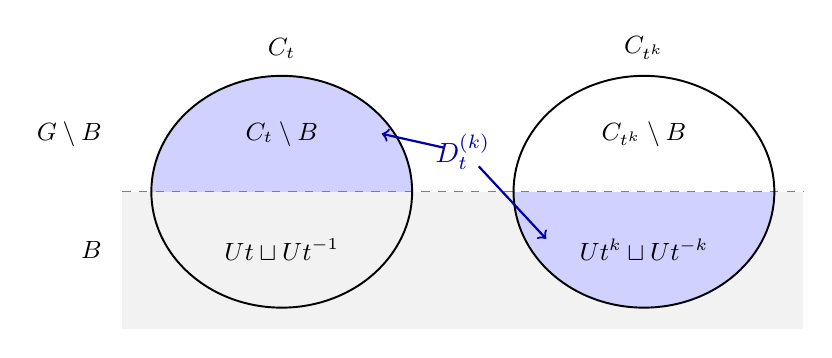
\begin{tikzpicture}[x=0.92cm,y=0.92cm,font=\small]
 % The lower band represents B; the upper region represents its complement.
 \fill[black!5] (-2.2,-1.9) rectangle (7.2,0);
 % Highlight precisely the part of C outside B and the part of C' inside B.
 \begin{scope}
  \clip (0,0) ellipse (1.8 and 1.6);
  \fill[blue!18] (-1.9,0) rectangle (1.9,1.7);
 \end{scope}
 \begin{scope}
  \clip (5,0) ellipse (1.8 and 1.6);
  \fill[blue!18] (3.1,-1.7) rectangle (6.9,0);
 \end{scope}
 \draw[dashed,black!50] (-2.2,0) -- (7.2,0);
 \draw[line width=0.7pt] (0,0) ellipse (1.8 and 1.6);
 \draw[line width=0.7pt] (5,0) ellipse (1.8 and 1.6);
 \node at (0,1.98) {$C_t$};
 \node at (5,1.98) {$C_{t^{k}}$};
 \node[anchor=east] at (-2.35,0.8) {$G\setminus B$};
 \node[anchor=east] at (-2.35,-0.8) {$B$};
 \node at (0,0.8) {$C_t\setminus B$};
 \node at (0,-0.8) {$U{t}\sqcup U{t^{-1}}$};
 \node at (5,0.8) {$C_{t^k}\setminus B$};
 \node at (5,-0.8) {$U{t^k}\sqcup U{t^{-k}}$};
 \node[text=blue!65!black,font=\normalsize] at (2.5,0.55) {$D_t^{(k)}$};
 \draw[->,blue!65!black,line width=0.8pt]
  (2.23,0.61) -- (1.38,0.8);
 \draw[->,blue!65!black,line width=0.8pt]
  (2.72,0.35) -- (3.65,-0.65);
\end{tikzpicture}
\caption{The two highlighted regions form the switched basic set $D_t^{(k)}=(C_t\setminus B)\sqcup(C_{t^k}\cap B)$.}
\label{fig:switched-class-Ct}
\end{figure}

Denote the resulting partition by $\D_k$. 
Our main result is as follows.
\begin{theorem}\label{thm:main}
For every $k\in(\mathbb Z/(q-1)\mathbb Z)^\times$, the partition $\D_k$ is a Schur partition of $G$, and the correspondence from each conjugacy class to its replacement preserves all structure constants.
If $k\not\equiv\pm1\pmod{q-1}$, the associated Cayley scheme is non-Schurian and therefore is not combinatorially isomorphic to $\X(G)$.
If $k\equiv\pm1\pmod{q-1}$, then $\D_k=\Cl(G)$.
\end{theorem}

Since $q-1\geq7$ is odd, $k=2$ always satisfies the nontriviality condition. 

The switching in \eqref{eq:switch-intro} is the analogue of the Borel switching construction in~\cite[Section~4]{HKK}. 
Two arguments establish the Suzuki-group case. 
First, all sets $gUt$, with $g\notin B$ and $t\in T$, are conjugate as subsets of $G$. 
Second, a local graph defined using the involution conjugacy class detects non-Schurity. 
Its cliques of size $q$ are cosets of centers of Sylow $2$-subgroups, and a trace calculation controls which of them survive the switching. 

\section{Preliminaries}

\subsection{Schur partitions and local graphs}

For a subset $A$ of a finite group, put$\clsum{A}=\sum_{a\in A}a\in\C G$.
A partition $\mathcal S$ of $G$ is a \emph{Schur partition} if it contains $\{1\}$, is closed under inversion, and its part sums span a subalgebra of $\C G$. 
Thus, for $A,B\in\mathcal S$,
\[
 \clsum{A}\clsum{B}=\sum_{C\in\mathcal S}c_{AB}^{C}\clsum{C}.
\]
The corresponding Cayley association scheme has relations
\[
 R_A=\{(x,y)\in G^2:yx^{-1}\in A\}\qquad(A\in\mathcal S).
\]
A bijection of parts preserving the constants $c_{AB}^C$ is an
\emph{algebraic isomorphism}. 
A \emph{combinatorial isomorphism} is a bijection of the underlying point sets that maps each relation onto a relation.
\emph{Separability} requires every algebraic isomorphism to be induced by a combinatorial one.

We use the local graph notion of~\cite[Definition~3.7]{HKK}. 
An element of $\mathcal S$ is called a \emph{basic set}. 
Let $X\in\mathcal S$ be a basic set, let $Y$ be a union of basic sets not containing $1$, and let $g\in G$. 
The \emph{local graph} $\Gamma_Y(X,g)$ has vertex set $R_X(g)=Xg$, with an arc from $a$ to $b$ when $ba^{-1}\in Y$. 
We abbreviate
\[
 \Gamma_Y(X):=\Gamma_Y(X,1).
\]
If $Y=Y^{-1}$, we regard this as an undirected graph.

\begin{lemma}\label{lem:local-schurian}
If the association scheme corresponding to $\mathcal S$ is Schurian, then every local directed graph $\Gamma_Y(X,g)$ is vertex-transitive.
\end{lemma}
\begin{proof}
Suppose the relations are the orbitals of a transitive permutation group $K$. 
The stabilizer $K_g$ is transitive on the relation neighborhood $R_X(g)=Xg$ and preserves every relation, hence also the adjacency relation defined by $Y$.
\end{proof}

In the proof of Theorem \ref{thm:main}, we exhibit a local graph on a switched basic set that is not vertex-transitive, thereby proving that the switched scheme is non-Schurian. 

Throughout this paper, let
\[
 \I=\{g\in G\setminus\{1\}:g^2=1\}
\]
be the set of involutions of $G$. 
As in~\cite[Section~4.2]{HKK}, we use $\Delta$ for the Cayley graph on the whole set $G$ in which $x$ and $y$ are adjacent when $yx^{-1}\in\I$. 

\subsection{Suzuki groups}
We include the matrix realization and Bruhat decomposition of the Suzuki groups, which are standard results; see Suzuki~\cite{Suzuki}, B\"a\"arnhielm~\cite[Section~2.1.1]{Baarnhielm}, and Breuillard--Green--Tao~\cite[Definition~3.1]{BGT}.
Note that \cite{BGT} uses the equivalent parameter $u(a,b+a^{\theta+1})$ for its unipotent matrices.

Set $\theta=2^{m+1}$, so that $a^{\theta^2}=a^2$ for $a\in\F_q$.
We use the standard matrix realization of the Suzuki group. 
For $a,b\in\F_q$ and $c\in\F_q^\times$, put
\begin{align}
 u(a,b)&=
 \begin{pmatrix}
 1&0&0&0\\
 a&1&0&0\\
 b&a^\theta&1&0\\
 a^{\theta+2}+ab+b^\theta&a^{\theta+1}+b&a&1
 \end{pmatrix},\label{eq:u-matrix}\\
 h(c)&=\diag(c^{\theta+1},c,c^{-1},c^{-\theta-1}),
 \qquad
 w=\begin{pmatrix}
 0&0&0&1\\0&0&1&0\\0&1&0&0\\1&0&0&0
 \end{pmatrix}.
 \label{eq:h-w}
\end{align}
Then $U=\{u(a,b):a,b\in\F_q\}$ and $T=\{h(c):c\in\F_q^\times\}$.
The standard structure theory gives
\begin{equation}\label{eq:bruhat}
 G=B\sqcup UTwU,\qquad B=U\rtimes T,
 \qquad wtw=t^{-1}\quad(t\in T),
\end{equation}
with unique parameters in each of the two cells. 
In particular,
\begin{equation}\label{eq:order}
 |G|=q^2(q^2+1)(q-1).
\end{equation}

Let $\Omega=G/B=\{gB:g\in G\}$.
We regard each left coset as a point, and let $G$ act on these points by left multiplication. 
We name two particular points
\[
 \infty:=B,\qquad 0:=wB.
\]

For a point $\alpha=gB$, let $B_\alpha=G_\alpha$ be its stabilizer. Explicitly,
\[
 B_\alpha=\{h\in G:hgB=gB\}=gBg^{-1}.
\]
We also define
\[
 U_\alpha:=gUg^{-1},\qquad
 Z_\alpha:=Z(U_\alpha)=gZ(U)g^{-1}.
\]
Thus the three subgroups $B_\alpha$, $U_\alpha$, and $Z_\alpha$ are obtained from $B$, $U$, and its center $Z(U)$ by the same conjugation. 
In particular, $U_\alpha$ is a normal Sylow $2$-subgroup of $B_\alpha$.
These definitions do not depend on the representative $g$ of the coset: every other representative has the form $gb$ with $b\in B$, and $U\lhd B$ gives
\[
 (gb)U(gb)^{-1}=gUg^{-1}.
\]
The same conclusion holds for $B_\alpha$ and $Z_\alpha$.
For the two distinguished points $\infty$ and $0$, the definitions give
\[
 \begin{aligned}
 B_\infty&=B,& U_\infty&=U,& Z_\infty&=Z(U),\\
 B_0&=wBw^{-1},& U_0&=wUw^{-1},& Z_0&=wZ(U)w^{-1}.
 \end{aligned}
\]

We call an element $x\in G$ a \emph{split semisimple element} if $x\in C_t$ for some $t\in T\setminus\{1\}$. We record the consequences of this action used below.

\begin{lemma}\label{lem:structure}
The following assertions hold.
\begin{enumerate}[label=\textup{(\roman*)},leftmargin=*]
\item The subgroup $U_\alpha$ acts regularly on $\Omega\setminus\{\alpha\}$. 
The action of $G$ on $\Omega$ is doubly transitive of degree $q^2+1$.
Every nonidentity element of $G$ fixes at most two points.
\item Distinct $U_\alpha$ intersect trivially. 
The involutions of $U_\alpha$ are exactly $Z_\alpha\setminus\{1\}$, and $|Z_\alpha|=q$.
The set $\I$ of all involutions of $G$ is a single conjugacy class.
\item If $t\in T\setminus\{1\}$, then $Ut$ is a single $U$-conjugacy orbit. Moreover,
\begin{equation}\label{eq:split-data}
 C_G(t)=T,\quad C_t\cap B=Ut\sqcup U{t^{-1}},\quad
 |C_t|=q^2(q^2+1).
\end{equation}
The equality $C_s=C_t$, for $s,t\in T\setminus\{1\}$, holds exactly when $s\in\{t,t^{-1}\}$.
\item If a split semisimple element $x$ fixes $\alpha$, then $xU_\alpha\subseteq x^G$. In particular, $xZ_\alpha\subseteq x^G$.
\end{enumerate}
\end{lemma}
\begin{proof}
Direct multiplication in \eqref{eq:u-matrix} gives
\begin{align}
 u(a,b)u(c,d)&=u(a+c,b+d+a^\theta c),\label{eq:U-product}\\
 u(a,b)^2&=u(0,a^{\theta+1}),\label{eq:U-square}\\
 h(c)^{-1}u(a,b)h(c)&=u(c^\theta a,c^{\theta+2}b).
 \label{eq:T-action}
\end{align}
The integers $\theta = 2^{m+1}$ and $\theta+2 = 2(2^{m}+1)$ are coprime to $q-1$. 
For the latter assertion, a common divisor of $2^m+1$ and $2^{2m+1}-1$ divides $1$, and $q-1$ is odd. 
If $t=h(c)\ne1$, then $c\ne1$, so $c^\theta\ne1$ and $c^{\theta+2}\ne1$. 
By \eqref{eq:T-action}, the equality $t^{-1}u(a,b)t=u(a,b)$ therefore forces $a=b=0$. Consequently,
\begin{equation}\label{eq:torus-centralizer-U}
C_U(t)=\{1\}\qquad(t\in T\setminus\{1\}).
\end{equation}

\textbf{(i)} \emph{Regular action}. 
The number of points in the coset action is
\[
 |\Omega|=[G:B]
 =\frac{q^2(q^2+1)(q-1)}{q^2(q-1)}=q^2+1.
\]
Since $T$ normalizes $U$ and $tw=wt^{-1}$, the Bruhat decomposition \eqref{eq:bruhat} can be written as $G=B\sqcup UwB$.
Hence every point other than $\infty$ has the form $uwB$ with $u\in U$. 
There are $q^2$ such points and $|U|=q^2$, so their representatives $u$ are unique. 
Under the identification \(u\leftrightarrow uwB\), \(U\) acts by left multiplication on itself, so the action is regular.
For \(\alpha=gB\), conjugate by $g$ to obtain the regular action of $U_\alpha=gUg^{-1}$ on $\Omega\setminus\{\alpha\}$. 
In particular, every nonidentity element of $U_\alpha$ fixes exactly the point $\alpha$.

\emph{Double transitivity.}
The action of $G$ on its cosets is transitive. 
Its stabilizer $G_\infty=B$ contains $U$, which is transitive on $\Omega \setminus \{\infty\}$. 
Thus $G$ is doubly transitive on $\Omega$.

\emph{The bound on fixed points.}
The group $T$ fixes $0=wB$.
Since $B=U \rtimes T$ and no nonidentity element of $U$ fixes $0$, the pointwise stabilizer of $\infty$ and $0$ is
\[
 G_{\infty,0}=T.
\]
For $t\in T$ and $u\in U$,
\[
 t\cdot(uwB)=(tut^{-1})wB.
\]
By uniqueness of the labels $u$, the point $uwB$ is fixed by $t$ exactly when $tut^{-1}=u$. 
If $t\ne1$, \eqref{eq:torus-centralizer-U} forces $u=1$, corresponding to the point $0$. 
Thus a nonidentity element of $T$ fixes precisely $\infty$ and $0$.
Now suppose a nonidentity element of $G$ fixed three distinct points.
By double transitivity, conjugate this element so that two of its fixed points become $\infty$ and $0$. The conjugate is a nonidentity element of $T$ and still fixes a third point, a contradiction.
This completes the proof of (i).

\textbf{(ii)} If $\alpha\ne\beta$, a nonidentity element in
$U_\alpha\cap U_\beta$ would fix both points, although a
nonidentity element of $U_\alpha$ fixes only $\alpha$. Hence
$U_\alpha\cap U_\beta=\{1\}$.

Equations \eqref{eq:U-product}--\eqref{eq:U-square} show that the
involutions in $U$ are exactly $u(0,b)$ with $b\ne0$, and that
\[
 Z(U)=\{u(0,b):b\in\F_q\}.
\]
Indeed, an element with $a\ne0$ cannot commute with every $u(c,0)$:
this would require $a^\theta c=c^\theta a$ for all $c\in\F_q$. 

Equation~\eqref{eq:T-action} shows that $T$ acts transitively
by conjugation on the involutions in $U$. Every involution
of $G$ lies in a Sylow $2$-subgroup, and every such subgroup
is conjugate to $U$. Hence every involution of $G$ is
conjugate to an involution in $U$, so all involutions of $G$
belong to a single conjugacy class. This proves (ii).

\textbf{(iii)} For $t\in T\setminus\{1\}$, the orbit--stabilizer theorem
and \eqref{eq:torus-centralizer-U} give
\[
 |\{utu^{-1}:u\in U\}|=|U:C_U(t)|=|U|.
\] 
This orbit is contained in $Ut$, by normality of $U$ in $B$, and hence equals $Ut$. 

In particular, every element of $B\setminus U$ is
$U$-conjugate to its image in $T$.
As proved above, the two fixed points of $t$ are $\infty$ and $0$.
Their pointwise stabilizer is $T$, and their setwise stabilizer
is $T\sqcup Tw$, because $w$ interchanges them. 
Every element of \(Tw\) inverts \(t\) and therefore cannot centralize \(t\), since \(t\) has odd order.
Thus $C_G(t)=T$.
Likewise, any conjugation carrying one nonidentity element of $T$ to another preserves this pair. Thus two elements \(s,t\in T\setminus\{1\}\) are conjugate in \(G\) if and only if \(s\in\{t,t^{-1}\}\).
No nonidentity element of $U$ is conjugate to $t$, since the former
has $2$-power order and the latter has odd order. Formula
\eqref{eq:split-data} and (iii) follow.

\textbf{(iv)} Choose $g\in G$ with $\alpha=gB$ and put
$y=g^{-1}xg$. Then $y\in B$, and its nontrivial odd order implies
$y\notin U$. Write $y=vt$ with $v\in U$ and
$t\in T\setminus\{1\}$. Since $U\lhd B$, we have
$yU=vtU=Ut$, which by (iii) is a single $U$-conjugacy orbit
containing $y$. Hence $yU\subseteq y^G$. Conjugating by $g$ gives
$xU_\alpha = g(yU) g^{-1}\subseteq y^G=x^G$.
\end{proof}

\section{Algebraic isomorphism}

\subsection{A uniform coset distribution}

The next observation explains the algebraic part of the construction.
It uses only \eqref{eq:bruhat} and the odd order of $T$.

\begin{lemma}\label{lem:uniform}
For every $g\in G\setminus B$ and $t\in T$, the subset $gUt$ is conjugate to $wU$. Consequently, for every conjugacy class $C$,
\begin{equation}\label{eq:uniform}
 |gUt\cap C|=|wU\cap C|.
\end{equation}
\end{lemma}
\begin{proof}
Write $g=u_1hw u_2$ with $u_1,u_2\in U$ and $h\in T$.
Normality of $U$ in $B$ gives
\[
 u_1^{-1}(gUt)u_1=hwUt=ht^{-1}wU.
\]
Conjugating the last set by $a\in T$ gives
\[
 a(ht^{-1}wU)a^{-1}=ht^{-1}a^2wU.
\]
Since $|T|$ is odd, the squaring map on \(T\) is bijective. We can choose $a$ with $a^2=th^{-1}$. This proves that $gUt$ is conjugate to $wU$.
\end{proof}

For conjugacy classes $C,E$, define, for $z\in B$,
\[
 F_{C,E}(z)=
 |\{(x,y)\in(C\setminus B)\times(E\setminus B):xy=z\}|.
\]

\Needspace{7\baselineskip}
\begin{lemma}\label{lem:outside-product}
The function $F_{C,E}$ is constant on $B\setminus U$.
\end{lemma}
\begin{proof}
Recall $B\setminus U = \sqcup_{t\ne 1} Ut$. For each $t\ne1$, conjugation by $U$ is transitive on $Ut$ and
preserves $C\setminus B$ and $E\setminus B$. Thus $F_{C,E}$ has a
constant value $f_t$ on $Ut$. Summing over $z\in Ut$ yields
\[
 q^2f_t=\sum_{x\in C\setminus B}|x^{-1}Ut\cap E|.
\]
Here $x^{-1}Ut\subseteq G\setminus B$, so there is no need to remove $B$ from $E$ in the summand. 
Lemma~\ref{lem:uniform} makes the right-hand side independent of $t$.
\end{proof}

\subsection{The counting argument}

Write $\sigma(t)=t^k$. For every conjugacy class $C$, denote its switched counterpart in $\D_k$ by $D_C$. 
Its intersection with $G\setminus B$ is unchanged.
If $C=C_t$, its intersection with $B$ is changed from
$Ut\sqcup U{t^{-1}}$ to $U{\sigma(t)}\sqcup U{\sigma(t)^{-1}}$.
Every other class meets $B$ in a subset of $U$, possibly empty, and is
unchanged.

\begin{proposition}\label{prop:algebraic}
For conjugacy classes $C,E,L$ and every $z\in D_L$,
\begin{equation}\label{eq:preservation}
 |\{(x,y)\in D_C\times D_E:xy=z\}|=c_{CE}^{L},
\end{equation}
where $c_{CE}^{L}$ is the corresponding intersection number of $\X(G)$. In particular, $C\mapsto D_C$ is an algebraic isomorphism.
\end{proposition}
\begin{proof}
The sets $D_C$ partition $G$ because $\sigma$ permutes the nonidentity
elements of $T$ and respects inversion. Their sizes are unchanged, the
identity singleton is unchanged, and
$D_{C^{-1}}=(D_C)^{-1}$. It remains to prove
\eqref{eq:preservation}.

First suppose $z\notin B$. In a factorization $xy=z$, it cannot happen that $x,y\in B$. 
The contribution with $x,y \not\in B$ is unchanged. 
The contribution from pairs with \(x\in A\subseteq B\) and \(y\in E\setminus B\) is
\[
 |\{a\in A:z^{-1}a\in E^{-1}\}|.
\]
Replacing $A=Ut\sqcup U{t^{-1}}$ by $U{\sigma(t)}\sqcup U{\sigma(t)^{-1}}$ preserves this count, by Lemma~\ref{lem:uniform}. 
For the case with \(x\not\in B\) and \(y\in B\), with second
factor $b\in B$, the condition $zb^{-1}\in C$ is equivalent to
$bz^{-1}\in C^{-1}$, and hence to $z^{-1}b\in C^{-1}$ by $z^{-1}$-conjugation.
Lemma \ref{lem:uniform} applies again. All contributions therefore agree with the
original ones at $z$, which belongs to $L$.

Now let $z\in B$. A factorization has either both factors in $B$ or
both outside $B$. If $z\in U$, take $z_0=z$. If $z\in Uv$ with
$v\ne1$, choose any $z_0\in U{\sigma^{-1}(v)}$. In both cases
$z_0\in L$. The contribution of two outside factors at $z$ after
switching equals the original contribution at $z_0$: for $z\in U$
this is immediate, and for $z\notin U$ it follows from
Lemma~\ref{lem:outside-product}.

For the contribution of two factors in $B$, use the quotient
homomorphism $B\longrightarrow T$. For $s,t,v\in T$ and $z\in Uv$,
\begin{equation}\label{eq:coset-product}
 |\{(x,y)\in Us\times Ut:xy=z\}|=
 \begin{cases}q^2,&st=v,\\0,&st\ne v.\end{cases}
\end{equation}
Also, for any $A\subseteq U$,
\begin{equation}\label{eq:mixed-coset}
 \begin{split}
 |\{(x,y)\in A\times Ut:xy=z\}|
 &=|\{(x,y)\in Ut\times A:xy=z\}|\\
 &=\begin{cases}|A|,&t=v,\\0,&t\ne v.\end{cases}
 \end{split}
\end{equation}
These identities follow by choosing the factor in the specified subset
and solving uniquely for the other factor. Products of two unchanged
subsets of $U$ are supported on $U$ and remain unchanged there.
Equations~\eqref{eq:coset-product}--\eqref{eq:mixed-coset} handle all
other cases, since $\sigma$ preserves the multiplication equations in
$T$. Thus the contribution inside $B$ at $z$ after switching agrees
with the original one at $z_0$.

Adding the contributions gives $c_{CE}^{L}$. This proves
\eqref{eq:preservation}, the Schur-partition assertion, and the
algebraic isomorphism.
\end{proof}

\section{Involution cliques and a trace bound}

Recall that $\Delta = \Gamma_{\I}(G)$ is the involution graph on $G$ and that the
local graph on a basic set $X$ is $\Gamma_{\I}(X)=\Delta[X]$.
The graph $\Delta$ is
undirected because involutions are self-inverse. Also recall that
$Z_\alpha=Z(U_\alpha)$ has order $q$.

\begin{lemma}\label{lem:cliques}
The maximum size of a clique in $\Delta$ is $q$. For any $x\in G$,
the cliques of size $q$ containing $x$ are precisely
\[
 xZ_\alpha\qquad(\alpha\in\Omega).
\]
These cliques are distinct for distinct $\alpha$.
\end{lemma}
\begin{proof}
Since $\I$ is invariant under conjugation, left translations are
automorphisms of $\Delta$: for $x,a,b\in G$,
\[
 (x^{-1}b)(x^{-1}a)^{-1}=x^{-1}(ba^{-1})x\in\I
 \quad\Longleftrightarrow\quad ba^{-1}\in\I.
\]
Let $K$ be a clique containing $x$. 
Its left translate $x^{-1}K$ is a clique containing $1$, so all its other vertices are involutions.
For any two distinct such vertices $a,b$, adjacency gives $ba^{-1}=ba\in\I$, and hence $ba=(ba)^{-1}=ab$. 
These vertices therefore generate an elementary abelian $2$-subgroup, contained in some Sylow $2$-subgroup $U_\alpha$. 
By Lemma~\ref{lem:structure}(ii), $x^{-1}K\subseteq Z_\alpha$. 
Thus $|K|\leq q$, and equality forces $x^{-1}K=Z_\alpha$, or equivalently $K=xZ_\alpha$.

Conversely, each $Z_\alpha$ is a clique of size $q$, since its nonidentity elements are involutions. 
Left translation shows that $xZ_\alpha$ is also a clique of size $q$ containing $x$.
Lemma \ref{lem:structure}(ii) implies that distinct $Z_{\alpha}$ intersect trivially, so the cosets \(xZ_\alpha\) are distinct as \(\alpha\) varies.
\end{proof}

\begin{lemma}\label{lem:trace}
If $x$ does not fix $\alpha\in\Omega$, then for every conjugacy
class $C$ of $G$,
\begin{equation}\label{eq:trace-bound}
 |xZ_\alpha\cap C|\leq2.
\end{equation}
\end{lemma}
\begin{proof}
By simultaneous conjugation, assume $\alpha=\infty$, so $x\notin B$.
Put $z(b)=u(0,b)$. From \eqref{eq:u-matrix},
\[
 z(b)=I+b(E_{31}+E_{42})+b^\theta E_{41},
\]
where $E_{ij}$ are matrix units.
Writing $x=(x_{ij})$, we obtain
\begin{equation}\label{eq:trace-polynomial}
 \tr(xz(b))=\tr(x)+(x_{13}+x_{24})b+x_{14}b^\theta.
\end{equation}
By the Bruhat decomposition, $x=u_1hw u_2$, so that $x_{14}=h_{11}\ne0$.

For $A\in\F_q$ and $B_0\in\F_q^\times$, each fiber of
$b\mapsto Ab+B_0b^\theta$ has at most two elements. Indeed, this
map is additive, and a nonzero element $d$ of its kernel satisfies
\[
 d^{\theta-1}=A/B_0.
\]
Recall the identity
$\gcd(2^r-1,2^s-1)=2^{\gcd(r,s)}-1$ for positive integers $r,s$,
which follows from the Euclidean algorithm applied to the exponents.
There is at most one such $d$, because
\[
 \gcd(\theta-1,q-1)
 =2^{\gcd(m+1,2m+1)}-1=1,
\]
the map \(d\mapsto d^{\theta-1}\) is a bijection of \(\mathbb F_q^\times\).
The trace is constant on $C$, so \eqref{eq:trace-polynomial} implies
\eqref{eq:trace-bound}.
\end{proof}

\begin{corollary}\label{cor:two-original-cliques}
Every vertex $x$ of the local graph $\Gamma_{\I}(C_t)$, with $t\ne1$,
lies in exactly two cliques of size $q$. They are $xZ_\alpha$ for
the two fixed points $\alpha$ of that vertex $x$.
\end{corollary}
\begin{proof}
If $x$ fixes $\alpha$, then $xZ_\alpha\subseteq C_t$ by
Lemma~\ref{lem:structure}(iv). If it does not, Lemma~\ref{lem:trace}
excludes this inclusion, since $q>2$. Now use
Lemma~\ref{lem:cliques} and the fact that a split semisimple element
has exactly two fixed points.
\end{proof}

\section{A local obstruction to Schurity}

Assume $k\not\equiv\pm1\pmod{q-1}$. Choose $t\in T$ such that
\begin{equation}\label{eq:moved-t}
 t^k\notin\{t,t^{-1}\};
\end{equation}
a generator of $T$ has this property. Abbreviate
\[
 C=C_t,\qquad C'=C_{t^k},\qquad D=D_t^{(k)}.
\]
The classes $C$ and $C'$ are distinct, and
\begin{equation}\label{eq:D-pieces}
 D\setminus B=C\setminus B,\qquad
 D\cap B=C'\cap B=U{t^k}\sqcup U{t^{-k}},\qquad D\cap C\cap B=\varnothing.
\end{equation}
Figure~\ref{fig:switched-class-Cprime} illustrates the two parts of $D$.

\begin{figure}[htbp]
\centering
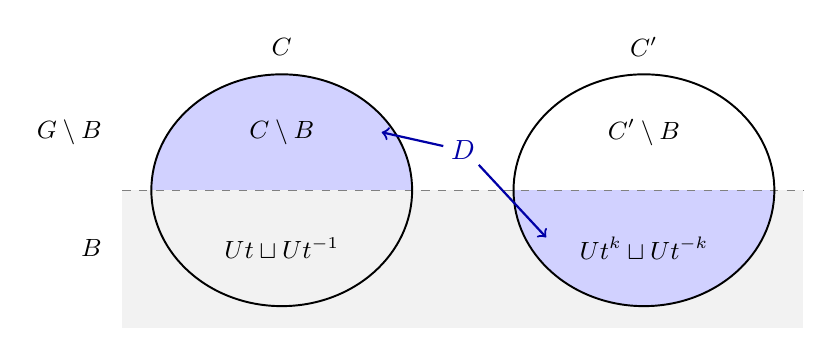
\begin{tikzpicture}[x=0.92cm,y=0.92cm,font=\small]
 % The lower band represents B; the upper region represents its complement.
 \fill[black!5] (-2.2,-1.9) rectangle (7.2,0);
 % Highlight precisely the part of C outside B and the part of C' inside B.
 \begin{scope}
  \clip (0,0) ellipse (1.8 and 1.6);
  \fill[blue!18] (-1.9,0) rectangle (1.9,1.7);
 \end{scope}
 \begin{scope}
  \clip (5,0) ellipse (1.8 and 1.6);
  \fill[blue!18] (3.1,-1.7) rectangle (6.9,0);
 \end{scope}
 \draw[dashed,black!50] (-2.2,0) -- (7.2,0);
 \draw[line width=0.7pt] (0,0) ellipse (1.8 and 1.6);
 \draw[line width=0.7pt] (5,0) ellipse (1.8 and 1.6);
 \node at (0,1.98) {$C$};
 \node at (5,1.98) {$C'$};
 \node[anchor=east] at (-2.35,0.8) {$G\setminus B$};
 \node[anchor=east] at (-2.35,-0.8) {$B$};
 \node at (0,0.8) {$C\setminus B$};
 \node at (0,-0.8) {$U{t}\sqcup U{t^{-1}}$};
 \node at (5,0.8) {$C'\setminus B$};
 \node at (5,-0.8) {$U{t^k}\sqcup U{t^{-k}}$};
 \node[text=blue!65!black,font=\normalsize] at (2.5,0.55) {$D$};
 \draw[->,blue!65!black,line width=0.8pt]
  (2.23,0.61) -- (1.38,0.8);
 \draw[->,blue!65!black,line width=0.8pt]
  (2.72,0.35) -- (3.65,-0.65);
\end{tikzpicture}
\caption{The two highlighted regions form the switched basic set
$D=(C\setminus B)\sqcup(C'\cap B)$.}
\label{fig:switched-class-Cprime}
\end{figure}

The involution class $\I$ is unchanged by switching and is a basic set
of both partitions. Thus $\Gamma_{\I}(C)$ and $\Gamma_{\I}(D)$ are the local
graphs on $C$ and $D$ in the original and switched schemes.

\begin{lemma}\label{lem:coset-B}
If $\alpha\ne\infty$, every left coset of $Z_\alpha$ meets $B$
in at most one element.
\end{lemma}
\begin{proof}
Every nonidentity element of $Z_\alpha$ fixes only $\alpha$, and
therefore $Z_\alpha\cap B=\{1\}$. If $xz_1,xz_2\in B$ with
$z_1,z_2\in Z_\alpha$, then
$(xz_1)^{-1}(xz_2)=z_1^{-1}z_2\in Z_\alpha\cap B$, whence $z_1=z_2$.
\end{proof}

\begin{lemma}\label{lem:fixed-only}
If $x\in D$ and $xZ_\alpha\subseteq D$, then $x$ fixes $\alpha$.
\end{lemma}
\begin{proof}
Suppose otherwise. If $\alpha=\infty$, then $x\notin B$ and the
entire coset $xZ_\infty$ is outside $B$. By \eqref{eq:D-pieces} it
would be contained in $C$, contrary to Lemma~\ref{lem:trace}.
If $\alpha\ne\infty$, Lemma~\ref{lem:coset-B} leaves at least
$q-1$ elements of this coset outside $B$. All would have to belong
to $C$, again contradicting Lemma~\ref{lem:trace}, because $q-1>2$.
\end{proof}

\begin{lemma}\label{lem:one-clique}
Every vertex of $D\cap B$ lies in exactly one clique of size $q$
in $\Gamma_{\I}(D)$.
\end{lemma}
\begin{proof}
Let $x\in D\cap B \subseteq C'$. 
Its two fixed points are $\infty$ and a point $\beta\ne\infty$. 
By Lemmas~\ref{lem:cliques} and \ref{lem:fixed-only}, the only possible cliques are $xZ_\infty$ and $xZ_\beta$. 
The first lies in the same $U$-coset as $x$, and hence in $D$, by \ref{lem:structure}(iii).

For the second, Lemma~\ref{lem:structure}(iv) gives $xZ_\beta\subseteq C'$. 
It meets $B$ only at $x$, by Lemma~\ref{lem:coset-B}. 
Its other $q-1$ vertices of this clique are in $C'\setminus B$, not contained in $D$.
\end{proof}

\begin{lemma}\label{lem:two-cliques}
At least $q^2(q-1)^2$ vertices of $D\setminus B$ lie in exactly two cliques of size $q$ in $\Gamma_{\I}(D)$.
\end{lemma}
\begin{proof}
By Corollary~\ref{cor:two-original-cliques}, every vertex of $C\setminus B$ lies in exactly two cliques of size $q$ in $\Gamma_{\I}(C)$. 
Such a clique survives in $\Gamma_{\I}(D)$ whenever it is disjoint from $B$. 
Conversely, for any clique $xZ_{\alpha}$ of size $q$ in $\Gamma_{\I}(D)$ through $x\in C\setminus B$, $x$ fixed $\alpha$, by Lemma~\ref{lem:fixed-only}. 
Then the entire coset $xZ_{\alpha}$ lies in $C$.

Count the original cliques that contain points both in $B$ and outside $B$. 
For each $r\in C\cap B$, its two original cliques are $rZ_\infty$, which is contained in $B$, and $rZ_\beta$, where $\beta$ is its other fixed point. 
The latter meets $B$ only at $r$, by Lemma \ref{lem:coset-B}. 
Consequently these crossing cliques are indexed without repetition by the elements of $C\cap B$. 
There are $2q^2$ of them, each with $q-1$ vertices outside $B$.

Thus at most $2q^2(q-1)$ vertices outside $B$ lie in a crossing clique. On the other hand,
\[
 |C\setminus B|=q^2(q^2+1)-2q^2=q^2(q^2-1).
\]
At least
\[
 q^2(q^2-1)-2q^2(q-1)=q^2(q-1)^2
\]
vertices lie in no crossing clique and therefore retain both of their original cliques. No additional cliques are possible by the first paragraph of the proof.
\end{proof}

\begin{proof}[Proof of Theorem~\ref{thm:main}]
Proposition~\ref{prop:algebraic} proves the Schur-partition and algebraic-isomorphism assertions. 
Under $k\not\equiv\pm1\pmod{q-1}$, Lemmas~\ref{lem:one-clique} and \ref{lem:two-cliques} give vertices of $\Gamma_{\I}(D)$ lying in different numbers of cliques of size $q$. 
Since this number is invariant under graph automorphisms, $\Gamma_{\I}(D)$ is not vertex-transitive.
Lemma~\ref{lem:local-schurian} proves that the switched scheme is non-Schurian. 
It cannot be combinatorially isomorphic to the Schurian scheme $\X(G)$. 
Finally, if $k\equiv\pm1\pmod{q-1}$, then $\D_k=\Cl(G)$, so the construction recovers $\X(G)$. 
\end{proof}

\begin{thebibliography}{9}

\bibitem{Baarnhielm}
H. B\"a\"arnhielm,
\emph{Algorithmic problems in twisted groups of Lie type},
Ph.D. thesis, Queen Mary, University of London, 2008.
\href{https://arxiv.org/abs/0805.3742}{arXiv:0805.3742}.

\bibitem{BGT}
E. Breuillard, B. Green, and T. Tao,
Suzuki groups as expanders,
\emph{Groups Geom. Dyn.} \textbf{5} (2011), no.~2, 281--299.
\href{https://arxiv.org/abs/1005.0782}{arXiv:1005.0782}.

\bibitem{HKK}
A. Higashitani, M. Kamiya, and H. Kurihara,
\emph{Twisted primitive group association schemes}, 2026.
\href{https://arxiv.org/abs/2608.16278}{arXiv:2608.16278}.

\bibitem{Suzuki}
M. Suzuki,
On a class of doubly transitive groups,
\emph{Ann. of Math. (2)} \textbf{75} (1962), no.~1, 105--145.
\href{https://doi.org/10.2307/1970423}{doi:10.2307/1970423}.

\end{thebibliography}
\end{document}
